\section*{Physique (13 points)}

\section{Ondes mécaniques et ondes lumineuses}
Les ondes mécaniques et les ondes lumineuses sont deux types d'ondes. La propagation de ces ondes est un phénomène naturel souvent observé dans la vie courante dans certains milieux. Selon les conditions, l'étude d'une telle propagation permet de mettre en évidence certains phénomènes physiques et déterminer quelques caractéristiques de ces ondes et du milieu de propagation.

Cet exercice vise~:
\begin{itemize}
    \item la détermination de certaines caractéristiques des ondes ultrasonores
          dans l'air~;
    \item la détermination de l'indice de réfraction d'un milieu transparent.
\end{itemize}

\subsection{Ondes ultrasonores}
\begin{minipage}{0.75\linewidth}
    On réalise une expérience en plaçant un émetteur $E$ d'ultrasons à une
    distance $d$ d'un récepteur $R$ d'ultrasons. L'émetteur $E$ émet à l'instant
    $t_{0}=0$ un signal ultrasonore de fréquence $N=\qty{40}{\kHz}$, ce signal
    est reçu par $R$ après un retard $\tau$.
    \begin{enumerate}
        \item Les ondes ultrasonores sont-elles des ondes mécaniques~?
              Justifier.
        \item Pour différentes valeurs de $d$, on mesure le retard $\tau$. Le
              graphe de la figure~\ref{fig:tau_d}, donne la variation de $\tau$
              en fonction de $d$.
        
              En exploitant le graphe, déterminer la valeur de la célérité $v$
              des ondes ultrasonores.
        \item Déduire la valeur de la longueur d'onde $\lambda$ des ultrasons.
    \end{enumerate}
\end{minipage}
\hfill
\begin{minipage}{0.23\linewidth}
    \begin{figure}[H]
        \centering
        \includegraphics[width=\textwidth]{2025-11-01_015224-}
        \caption{}
        \label{fig:tau_d}
    \end{figure}
\end{minipage}







Partie 2 : Indice de réfraction d'un milieu transparent\\
On réalise la diffraction d'une lumière monochromatique dans l'air et dans un milieu transparent d'indice $n$ en utilisant le dispositif schématisé sur la figure 2.\\
Le dispositif comporte un laser, un fil fin de diamètre $a$ et un écran placé à la distance $D$ du fil. On désigne par $\theta$ l'écart angulaire de diffraction.

Donnée: Pour $\theta$ très petit $\tan \theta \approx \theta(\mathrm{rad})$

\begin{enumerate}
  \item Définir une lumière monochromatique.
  \item Le dispositif est placé dans l'air, le laser émet une radiation monochromatique de longueur d'onde $\lambda_{0}$.\\
La largeur de la tache centrale observée sur l'écran est $L_{0}=1,9 \mathrm{~cm}$.\\
Exprimer $\lambda_{0}$ en fonction de $a, L_{0}$ et $D$.\\
\includegraphics[width=\textwidth]{2025_05_10_39ba27a3e62f3257e522g-4}
\end{enumerate}

Figure 2\\
3. On refait la même expérience en plaçant le fil et l'écran dans le milieu transparent d'indice $n$ en gardant la même distance $D$. La largeur de la tache centrale observée sur l'écran est $L=1,4 \mathrm{~cm}$.\\
Trouver l'expression de l'indice $n$ en fonction de $L_{0}$ et $L$. Calculer sa valeur.

\section*{Exercice 2 (5 points): Charge et décharge d'un condensateur}
Le condensateur, la bobine et le conducteur ohmique sont des composants électroniques dont le comportement diffère selon les circuits électriques où ils se trouvent. Dans des conditions expérimentales, l'association de certains d'entre eux peut engendrer des phénomènes électriques tels que la charge du condensateur, sa décharge selon différents régimes, les oscillations électriques et impacte le bilan énergétique dans ces circuits.

\section*{Cet exercice vise :}
\begin{itemize}
  \item l'étude de la charge d'un condensateur ;
  \item l'étude des oscillations électriques libres dans un circuit RLC série.
\end{itemize}

On considère le montage de la figure 1 comportant :

\begin{itemize}
  \item un générateur idéal de tension de force électromotrice $E$;
  \item un condensateur de capacité $C=1 \mu \mathrm{~F}$;
  \item un conducteur ohmique de résistance $R_{0}$ et un autre de résistance $R$ réglable ;
  \item une bobine d'inductance $L$ et de résistance négligeable ;
  \item un interrupteur $K$ à double position.
\end{itemize}

\begin{enumerate}
  \item À l'instant $t_{0}=0$, on place l'interrupteur $K$ en position (1). Un système d'acquisition convenable permet d'obtenir la courbe représentant la variation de la charge $q$ du condensateur en fonction du temps (figure 2).
\end{enumerate}

\begin{center}
\begin{tabular}{|l|l|}
\hline
\includegraphics[width=\textwidth]{2025_05_10_39ba27a3e62f3257e522g-5}
 & \includegraphics[width=\textwidth]{2025_05_10_39ba27a3e62f3257e522g-5(1)}
 \\
\hline
Figure 1 & Figure 2 \\
\hline
\end{tabular}
\end{center}

1.1. Établir l'équation différentielle vérifiée par la charge $q$ du condensateur.\\
1.2. En exploitant le graphe de la figure 2 , déterminer la valeur de :

\begin{itemize}
  \item la force électromotrice $E$;
  \item la constante de temps $\tau$;
  \item la résistance $R_{0}$;
  \item l'intensité maximale $I_{0}$ du courant électrique.\\
1.3. Recopier, sur votre copie, le numéro de la question et écrire la lettre correspondante à la proposition vraie.
\end{itemize}

L'expression de la charge $q$ en coulomb est :

\begin{center}
\begin{tabular}{|c|c|c|c|}
\hline
$\mathbf{A}$ & $q(t)=5.10^{-6} .\left(1-e^{-10^{2} . t}\right)$ & $\mathbf{B}$ & $q(t)=6.10^{-6} .\left(1-e^{-10^{5} . t}\right)$ \\
\hline
$\mathbf{C}$ & $q(t)=5.10^{-6} . e^{-10^{4} . t}$ & $\mathbf{D}$ & $q(t)=5.10^{-6} .\left(1-e^{-10^{4} . t}\right)$ \\
\hline
\end{tabular}
\end{center}

\begin{enumerate}
  \setcounter{enumi}{1}
  \item Lorsque le condensateur est totalement chargé, on bascule l'interrupteur en position (2) à un instant pris comme nouvelle origine de temps $t_{0}=0$.
\end{enumerate}

Les courbes (1), (2) et (3) de la figure 3 (page 6/7) représentent la tension $u_{C}(t)$ aux bornes du condensateur pour trois valeurs de la résistance $R: R_{1}=100 \Omega, R_{2}=2 \mathrm{k} \Omega$ et $R_{3}=20 \mathrm{k} \Omega$.\\
2.1. Attribuer chaque courbe de la figure 3 à la résistance correspondante.\\
2.2. Nommer les régimes d'oscillations correspondants aux courbes (2) et (3).\\
2.3. On considère le point $S$ de la courbe (2) de coordonnées : $t_{S}=12,6 \mathrm{~ms} ; u_{C S}=2,6 \mathrm{~V}$\\
a. Déterminer la valeur de la pseudo-période $T$ des oscillations.\\
b. Déduire la valeur de l'inductance $L$ (on suppose que la pseudo-période $T$ est égale à la période propre $T_{0}$ des oscillations libres non amorties).\\
c. Calculer la variation de l'énergie totale $\Delta \mathcal{E}$ entre l'instant $t_{0}=0$ et l'instant $t_{s}$.\\
2.4. On veut obtenir des oscillations électriques sinusoïdales non amorties. Sur quelle valeur doit-on régler la résistance $R$ ?\\
\includegraphics[width=\textwidth]{2025_05_10_39ba27a3e62f3257e522g-6(1)}

Figure 3


\section*{Exercice 3 (5 points): Mouvement d'un solide}
La translation rectiligne d'un solide est un type de mouvement. L'étude de ce type de mouvement dépend de la nature des actions mécaniques appliquées et des conditions initiales et peut se faire par une étude dynamique ou énergétique, ce qui permet d'établir les équations qui gèrent le mouvement et de déterminer certaines de ses grandeurs caractéristiques.\\
Cet exercice vise :

\begin{itemize}
  \item l'étude du mouvement d'un solide soumis à des forces constantes;
  \item l'étude du mouvement d'un solide soumis à une force variable.
\end{itemize}

\section*{Partie 1 : Étude d'un mouvement de translation}
On lance vers le haut, depuis la position $O$, avec une vitesse initiale $\overrightarrow{v_{0}}$, suivant la ligne de plus grande pente d'un plan incliné d'un angle $\alpha$ par rapport à l'horizontal, un solide ( $S$ ) de masse $m$ (figure 1). Le solide ( $S$ ) arrive en $A$ après avoir parcouru la distance $O A=L$, puis redescend. Tout au long de son mouvement, ( $S$ ) est soumis à des frottements modélisés par une force constante $\vec{f}$ de sens opposé au sens du vecteur vitesse.\\
On étudie le mouvement du centre d'inertie $G$ du solide ( $S$ ) dans un repère ( $O, \ex$ ) lié à la Terre supposé galiléen. L'abscisse de $G$ à $t_{0}=0$\\
\includegraphics[width=\textwidth]{2025_05_10_39ba27a3e62f3257e522g-6}

Figure 1 est $x_{G}=x_{0}=0$.\\
Données : $m=200 \mathrm{~g}$; $v_{0}=3 \mathrm{~m} . \mathrm{s}^{-1} ; \sin \alpha=0,1 ; \quad g=10 \mathrm{~m} . \mathrm{s}^{-2} ; L=3 \mathrm{~m}$

\begin{enumerate}
  \item En appliquant la deuxième loi de Newton, montrer que l'équation différentielle vérifiée par $x_{G}$ lors de la montée s'écrit : $\frac{d^{2} x_{G}}{d t^{2}}=-\frac{f}{m}-g \cdot \sin \alpha$.\\
Déduire, en justifiant, la nature du mouvement de $(S)$.
  \item Le solide ( $S$ ) atteint la position $A$ à l'instant $t_{1}=2 \mathrm{~s}$. Déterminer pour cette phase la valeur de l'accélération $a_{G}$ et celle de l'intensité $f$.
  \item Lors de la descente, on choisit l'instant de départ de la position $A$ comme nouvelle origine de temps $t_{0}=0$.\\
3.1. Montrer que l'équation horaire du mouvement de ( $S$ ) lors de la descente est : $x(t)=-0,25 . t^{2}+3(m)$.\\
3.2. Déterminer la valeur algébrique de la vitesse de ( $S$ ) lorsqu'il repasse par $O$.
\end{enumerate}

\subsection{Étude d'un système oscillant}
\begin{minipage}{0.64\linewidth}
    Le solide $(S)$ de masse $m=\qty{200}{\gram}$ est fixé à un ressort
    horizontal à spires non jointives, de masse négligeable et de raideur $K$. À
    l'équilibre, le centre d'inertie $G$ de $(S)$ coïncide avec l'origine du
    repère ($O,\ex$) lié à la Terre supposé galiléen
    (figure~\ref{fig:solide_ressort}). Tous les frottements sont négligeables.
\end{minipage}
\hfill
\begin{minipage}{0.35\linewidth}
\begin{figure}[H]
    \centering
    \begin{tikzpicture}
    \node[inner sep=0pt,minimum width=4.5cm,minimum height=3mm,
        top color=black!70] (sol) {};
    % Axe xx'
    \coordinate (O) at ($(sol.south west)!.8!(sol.south east)$);
    \draw[-Latex] (sol.south west)
        node[below right,inner xsep=0pt] {$x^{\prime}$} -- (O)
        node[below=0.4mm] {$O$} -- (sol.south east) -- ++(0.7,0)
        node[below left,inner xsep=0pt,inner ysep=2mm] {$x$};
    % Fixed
    \node[inner sep=0pt,draw,minimum width=3mm,minimum height=7mm,
        anchor=south,pattern=north west lines,
        thick] (fix) at ([xshift=3mm,yshift=0.4pt]sol.north west) {};
    % Solide (S)
    \node[inner sep=0pt,draw,minimum width=7mm,minimum height=7mm,
        anchor=south,rounded corners=2pt,thick,label=$\mathrm{(S)}$,
        fill=lightgray] (S) at
        ([yshift=0.4pt]O |- sol.north) {};
        %([xshift=-6mm,yshift=0.4pt]sol.north east) {};
    \node[inner sep=1pt,circle,fill,
        label={[right=-0.8mm,font=\scriptsize]:$G$}] (G) at (S.center) {};
    \draw[{Rectangle[length=1pt,width=4pt]}-{Stealth[length=5pt]},
        thick] (O) -- ++(0.8,0)
        node[below left,inner xsep=0pt] {$\ex$};
    % Ressort
    \draw[decoration={
          coil,
          aspect=0.3,
          segment length=2.0mm,
          amplitude=2.4mm,
          pre length=1mm,
          post length=1mm},
          decorate,thick,black] (fix.east) -- (S.west);
\end{tikzpicture}

    \caption{}
    \label{fig:solide_ressort}
\end{figure}
\end{minipage}

On écarte ($S$) de sa position d'équilibre dans le sens positif d'une
distance $X_{m}$ et on l'abandonne sans vitesse initiale à $t_{0}=0$.

Le solide ($S$) effectue alors un mouvement de translation rectiligne
sinusoïdal de période propre $T_{0}$.
\begin{enumerate}
    \item Le solide ($S$) effectue 20 oscillations pendant la durée
          $\Delta t=\qty{12,6}{\second}$.

          Vérifier que $K=\qty{20}{\newton\per\meter}$.
\end{enumerate}
\begin{minipage}{0.64\linewidth}
    \begin{enumerate}
        \setcounter{enumi}{1}
        \item On choisit l'état où le ressort n'est pas déformé comme état de
              référence de l'énergie potentielle élastique $E_{pe}$ et le plan
              horizontal contenant $G$ comme état de référence de l'énergie
              potentielle de pesanteur $E_{pp}$.
    
              La courbe de la figure~(\ref{fig:Ec_de_t}) représente le diagramme
              d'énergie cinétique $E_{c}=f(t)$ du solide.
    
              En exploitant le diagramme, déterminer les valeurs de~:
              \begin{enumerate}
                  \item l'énergie mécanique $E_{m}$.
                  \item l'amplitude $X_{m}$.
                  \item l'abscisse $x_{1}$ du centre d'inertie $G$ de ($S$) à
                        l'instant $t_{1}=\qty{1,2}{\second}$.
              \end{enumerate}
    \end{enumerate}
\end{minipage}
\hfill
\begin{minipage}{0.35\linewidth}
 \begin{figure}[H]
    \centering
    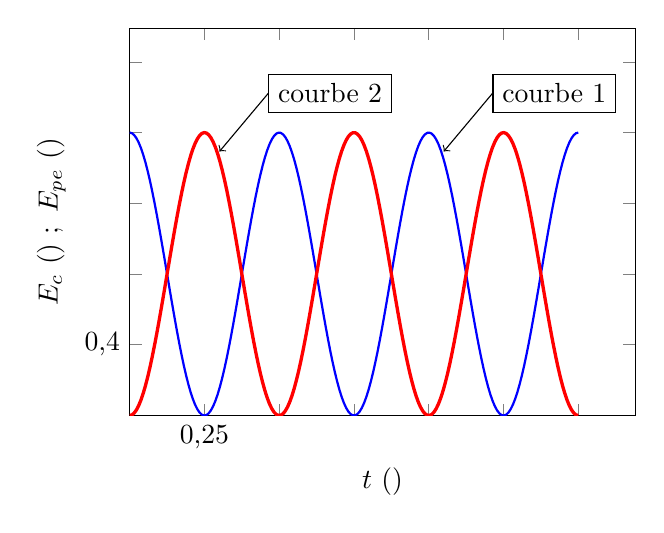
\begin{tikzpicture}
        \def\Xm{0.02}
        \def\T{1}
        \def\K{8}
        \pgfmathpi\let\pi=\pgfmathresult
        \begin{axis}[
                xmin=0,xmax=1.69,
                ymin=0,ymax=2.19,
                width=8cm,height=6.5cm,
                trig format plots=rad,
                xtick distance=0.25, ytick distance=0.4,
                xticklabels={,,{0,25}}, yticklabels={,,{0,4}},
                xlabel=$t~(\unit{\second})$,
                ylabel=$E_{c}~(\unit{\mJ})~;~E_{pe}~(\unit{\mJ})$,
            ]
            \addplot[domain=0:1.5,samples=200,thick,blue]
                {0.5*\K*\Xm*\Xm*cos(2*pi/\T*x)*cos(2*pi/\T*x)*1e3}
                coordinate[pos=0.68] (c1);
            \addplot[domain=0:1.5,samples=200,very thick,red]
                {0.5*\K*\Xm*\Xm*sin(2*pi/\T*x)*sin(2*pi/\T*x)*1e3}
                coordinate[pos=0.18] (c2);
        \end{axis}
        \draw[<-,shorten <=1pt] (c1) -- ++(50:1) node[right,draw] {courbe~1};
        \draw[<-,shorten <=1pt] (c2) -- ++(50:1) node[right,draw] {courbe~2};
    \end{tikzpicture}
    \caption{}
    \label{fig:Ec_de_t}
\end{figure}   
\end{minipage}




